\documentclass[UTF8,9pt]{ctexart}
\usepackage{../../template/homeworkTEMP/hw} 
\setcounter{secnumdepth}{0}
    \title{The 4th Homework of Optics}  
\begin{document}
\maketitle
\section{3-1}
双缝干涉中条纹间距为
$$\Delta x=\f{\lambda D}{d}$$
代入$D=3000mm,\ d=0.1mm,\ \lambda=486.1\times10^{-6}mm,589.3\times10^{-6}mm,656.3\times10^{-6}mm$:
$$\Delta x_F=14.6mm$$
$$\Delta x_D=17.7mm$$
$$\Delta x_C=19.7mm$$
\section{3-4}
当两股等长时,相位差$\phi=0$
当拉长$d$后,B方向长度增加$2d$,且相位差$\phi=\pi$,即此时波程相差$\lambda/2$,即:
$$\lambda/2=2d=2\times 16cm \Rightarrow \lambda=64cm$$
\section{3-5}
\subsection{(1)}
\begin{center}
	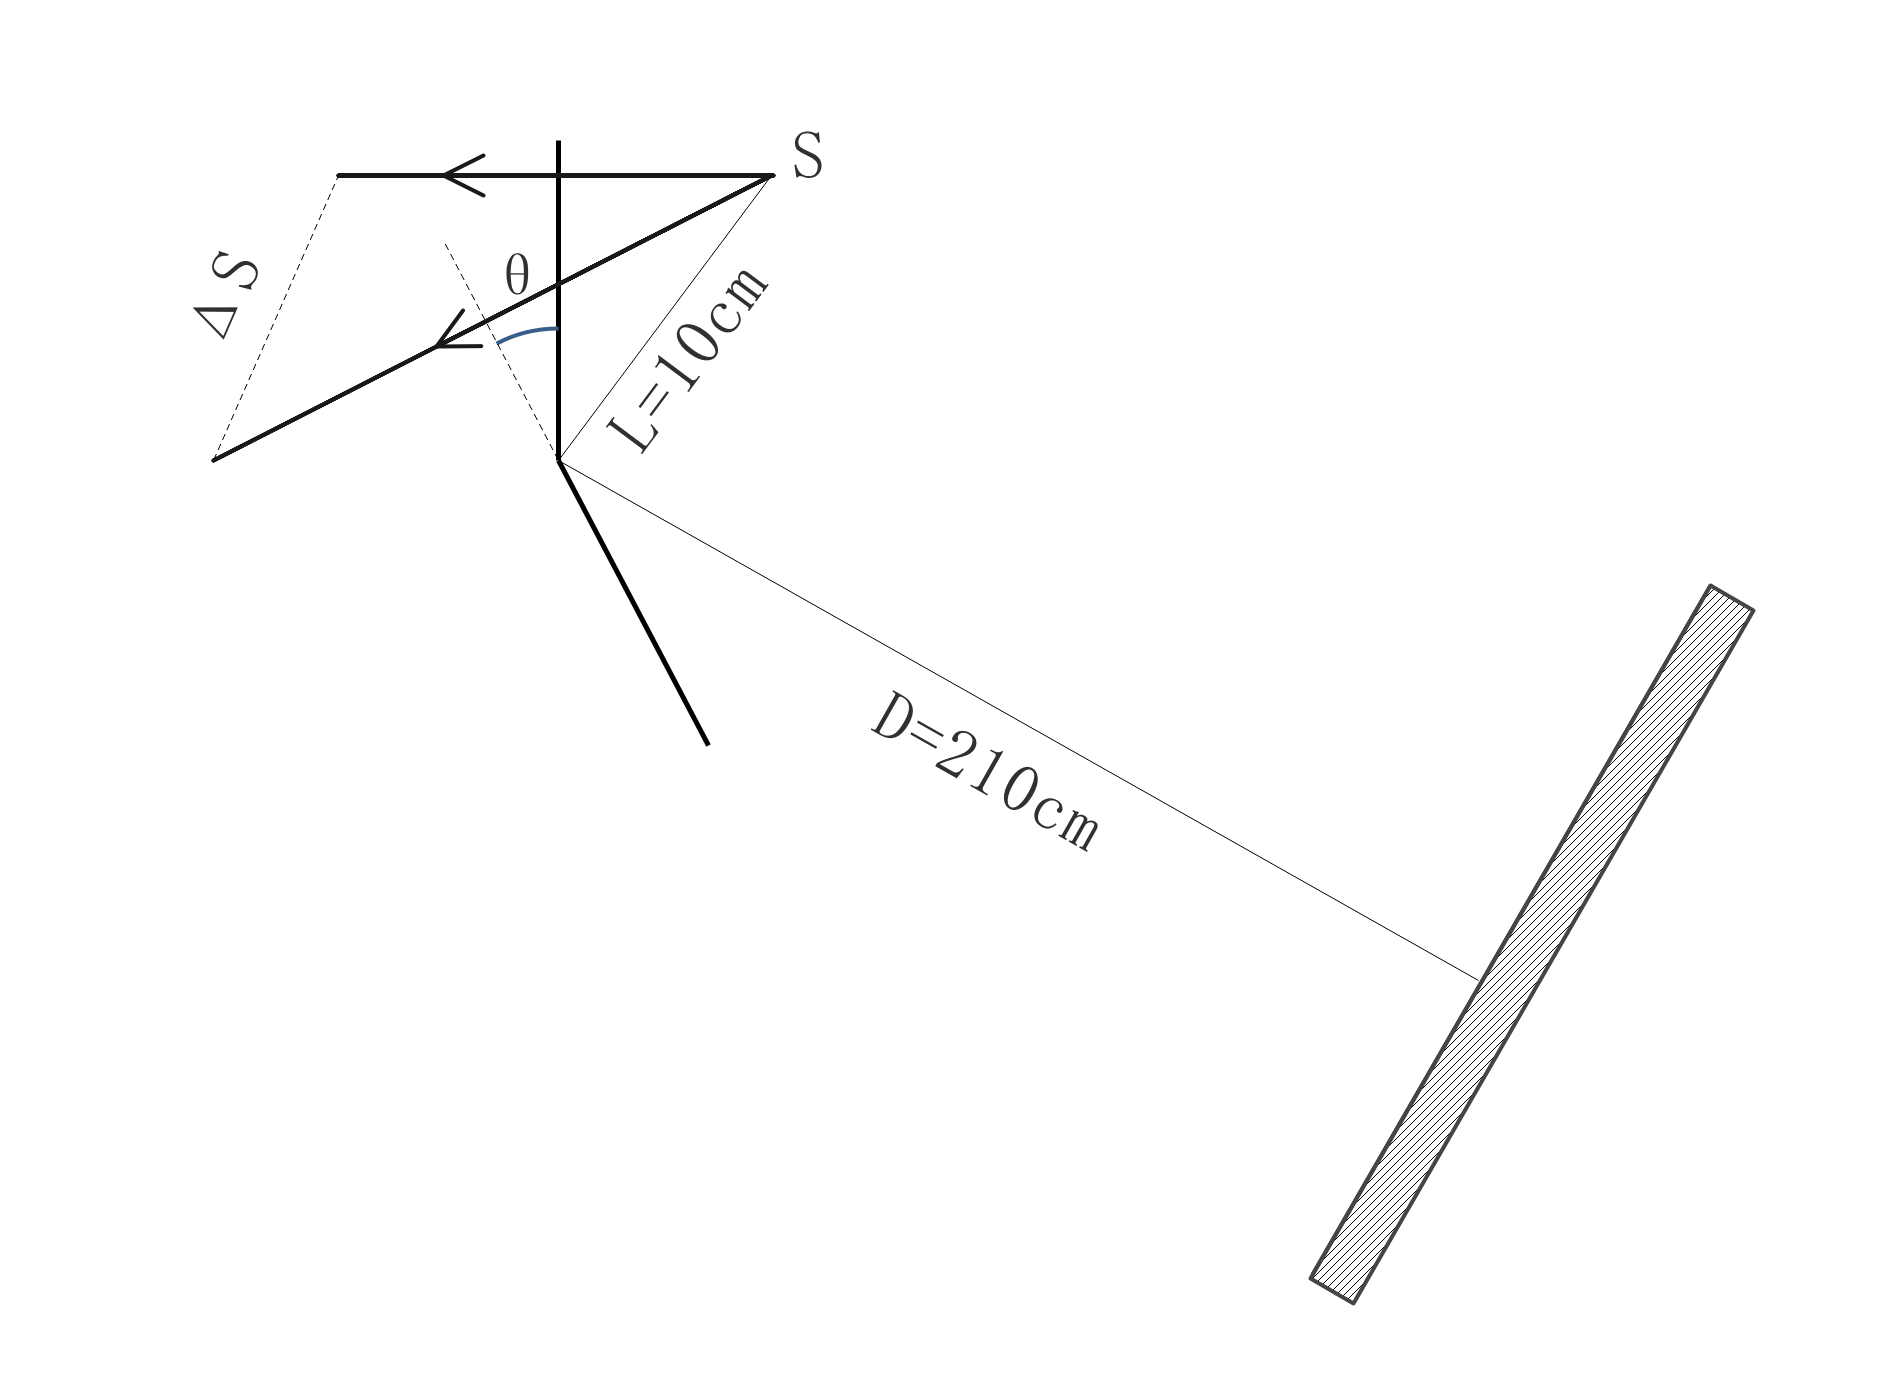
\includegraphics[scale=0.1]{1.png}\\
\end{center}
$$\Delta S=2L\sin\theta=20 \sin \left(\frac{\pi }{540}\right)cm$$
条纹间距
$$\Delta x=\f{\lambda (R+D)}{\Delta S}=\frac{3 \left(210+10 \cos \left(\frac{20 \pi }{60\ 180}\right)\right)}{5000 \left(20 \sin \left(\frac{\pi }{540}\right)\right)}=1.13mm$$
\subsection{(2)}
两虚光源与平面镜交点连线与光屏与平面镜交点连线所成夹角为$\theta$\\
则能形成条纹的范围为:
$$L_0=2D\tan\theta=24.43mm$$
条纹数量为:
$$N=L_0/\Delta x\approx 22$$
	\subsection{(3)}
此时光源间距$\Delta S$扩大一倍,光源到光屏距离$D'$增加少许,条纹间距减半,条纹数量翻倍:
$$\Delta S'=2L'\sin\theta=40 \sin \left(\frac{\pi }{540}\right)cm$$
$$\Delta x'=\frac{3 \left(210+20 \cos \left(\frac{20 \pi }{60\ 180}\right)\right)}{50000 \left(40 \sin \left(\frac{\pi }{540}\right)\right)}=0.59mm$$
$$N=L_0/\Delta x'\approx 44$$
\subsection{(4)}
若光源横向移动,光源间距不变,因此条纹间距,数量均不变,但双像中垂线与光屏交点会移动,导致零级位置转动角$\delta x=\f{C}{B}\delta s$。在光屏上的表现就是所有条纹沿垂直于条纹方向反向平移。
\subsection{(5)}
题述即要求条纹平移低于$\Delta x$,光源的极限宽度为:
$$b_0=\f{R}{D}\Delta x=0.054mm$$
\section{3-6}
入射角$$i=3'30''=\frac{7 \pi }{21600}$$
则可计算出折射角为$$j=\arcsin\left(n\sin i\right)\approx 0.00152716$$
折射光线与水平夹角为$$\alpha=j-i \approx 0.000509055$$
$\Rightarrow $屏幕上出现条纹的长度为$$L=5m\tan \times \alpha \times 2=5.09055mm$$
条纹间距为$$\Delta x=\f{\lambda D}{d}=\lambda \cot2\alpha=0.491106mm$$
根据上面的计算可以得到条纹数量$$N=\f{L}{\Delta x}\approx 10$$
\section{3-8}
\subsection{(1)}
\begin{center}
	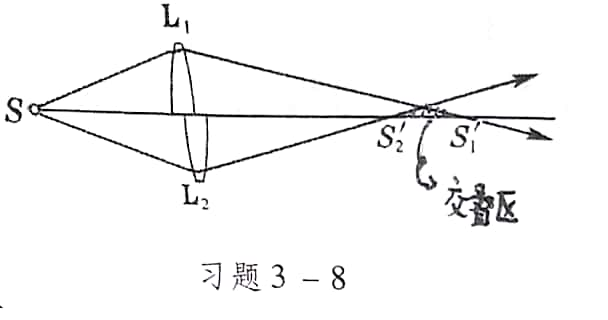
\includegraphics[scale=0.4]{2.jpg}\\
\end{center}
\subsection{(2)}
呈现为明暗交替的同心圆。
\subsection{(3)}
$L_1$所成像位置:
$$x'_1=s_1+s'_1=60+\ff{\ff{f}-\ff{s_1}}=120cm$$
$L_2$所成像位置:
$$x'_2=s_2+s'_2=62+\ff{\ff{f}-\ff{s_2}}=120.125cm$$
则中点距离为:
$$s'_{ave}=\f{x'_1+x'_2}{2}-62=58.0625$$
\subsection{(3)}
\begin{center}
	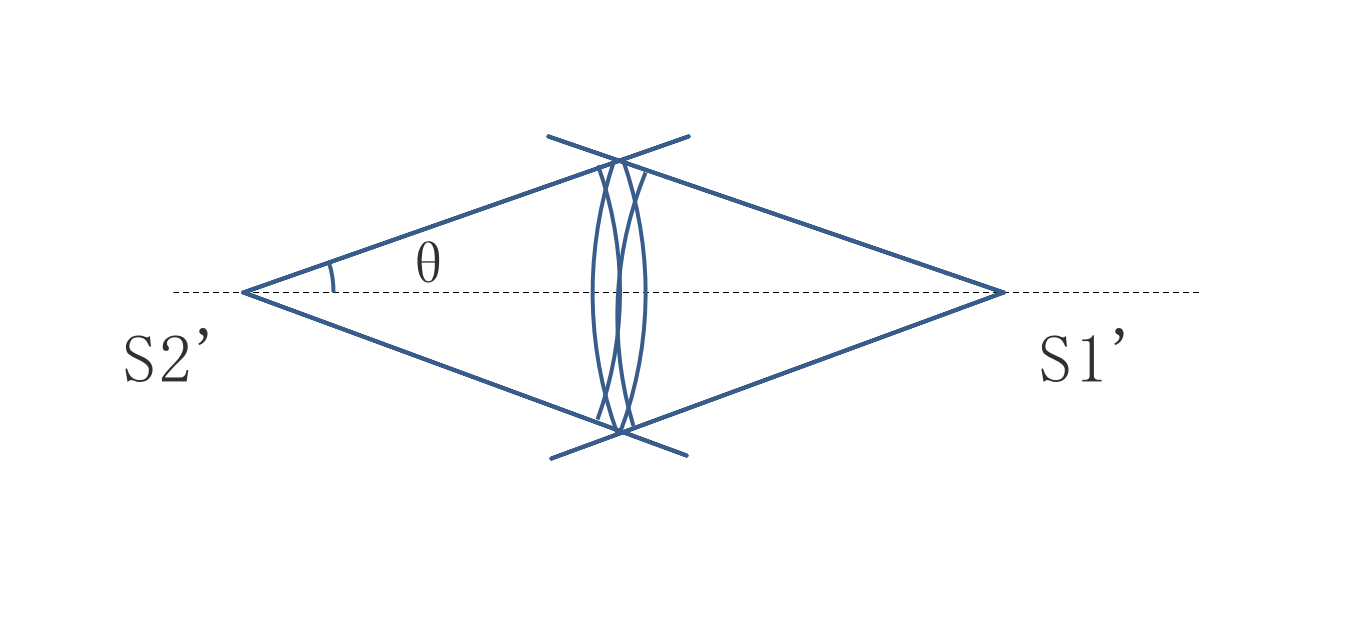
\includegraphics[scale=0.4]{3.png}\\
\end{center}
如图,设条纹间距为$\Delta x$,则在相差一个波长的两处:
$$\cos\theta=\f{x_2'-x_1'}{2}/(\f{x_2'-x_1'}{2}+\lambda)$$
$$\tan\theta=\Delta y/\f{x_2'-x_1'+\lambda}{2}$$
$\Rightarrow $条纹间距为:
$$\Delta y=\sqrt{(\f{x_2'-x_1'}{2}+\lambda)^2-(\f{x_2'-x_1'}{2})^2}$$
$$=0.007cm$$
\section{3-9}
\subsection{(1)}
此时$S_1$方向容器内光程增加,因此外部光程需减小,条纹上移。
\subsection{(2)}
增加氯气后容器内增加的光程:
$$L_i=l(n_{Cl}-n_{air})$$
外部减少的光程:
$$L_o=20\lambda n_{air}$$
二者相等:
$$l(n_{Cl}-n_{air})=20\lambda n_{air} \Rightarrow n_{Cl}=1.000865$$
\section{3-14}
\subsection{(1)}
条纹间距与顶角的关系为:
$$\Delta x=\f{\lambda}{2\alpha}$$
$$\alpha=\f{\Delta h}{l}$$
$$\Rightarrow \Delta h=0.029465mm$$
按压$G_1, G_2$中央位置,较长的一块倾角会变大,条纹变密。
\subsection{(2)}
由上面的推导可以知道$T$与$G_2$间的倾角更大
$$\alpha_1=0.0005893$$
$$\alpha_2=0.000982167$$
工件$G_2$有法线朝右上角的倾角$\Delta \alpha=0.000393=1.351'$
\section{3-16}
\subsection{(1)}
可以将干涉分解为一次从半反射膜到P区表面的干涉和P区表面到半导体表面的干涉,前者沿横向的轴翻转,因此产生了横向的条纹,后者沿纵向的轴反转,因此产生了纵向的条纹,最后形成的斜向条纹为两个干涉条纹的叠加。
\subsection{(2)}
总倾角为:
$$\alpha=\f{\lambda}{2\Delta x}=0.001375$$
$AB$之间共有4.5条条纹。可以得到半反射膜翻转角度:
$$\alpha_b=\f{\lambda}{2\Delta x}=0.001125$$
则半导体倾角为:
$$\alpha_a=\sqrt{0.001375^2-0.001125^2}=0.00079$$
节深$$x_j=l_{AB}\tan\alpha_a=0.00151mm$$
\subsection{(3)}
该方法没有准确判断半反射膜与半导体接触位置的困难。
\section{3-20}
\subsection{(1)}
由于入射光线靠近法线,强度反射率$R$满足:
$$R = \left( \frac { n _ { 1 } - n _ { 2 } } { n _ { 1 } + n _ { 2 } } \right) ^ { 2 }=0.298$$
\subsection{(2)}
$$n_{film}=\sqrt{n_{glass}n_{air}}=1.844$$
$$h=(\ff{4}+\f{k}{2})\f{\lambda}{n_{film}}=126.091 + 252.182 k\ nm(k=0,1,2...)$$
取k=0,
$$h=\ff{4}\f{\lambda}{n_{film}}=126 nm$$
\subsection{(3)}
此时仍能保持$n_{glass}>n_{MgF_2}>n_{air}$,能增透,\\
第一次玻璃-膜反射,振幅反射率为:
$$r_1=\f{n_{glass}-n_{film}}{n_{glass}+n_{film}}=0.42259$$
第一次反射光振幅为:
$$A_1=r_1A_0=0.42259A_0$$
第二次膜-空气反射,振幅反射率为:
$$r_2=\f{n_{film}-n_{air}}{n_{film}+n_{air}}=0.15967$$
第二次反射光经过2次透射1次反射,振幅为:
$$A_2=\sqrt{(1-r_1^2)}r_2\sqrt{(1-r_1^2)}A_0=0.13115A_0$$
由于二者反相,可得到反射光强为:
$$I_r=(A_2-A_1)^2=0.085A_0^2$$
则反射率为:
$$R=\f{I_r}{I}=8.5\%$$
\subsection{(4)}
此时仍能保持$n_{glass}>n_{ZnS}>n_{air}$,能增透,\\
第一次玻璃-膜反射,振幅反射率为:
$$r_1=\f{n_{glass}-n_{film}}{n_{glass}+n_{film}}=0.182609$$
第一次反射光振幅为:
$$A_1=r_1A_0=0.182609A_0$$
第二次膜-空气反射,振幅反射率为:
$$r_2=\f{n_{film}-n_{air}}{n_{film}+n_{air}}=0.402985$$
第二次反射光经过2次透射1次反射,振幅为:
$$A_2=\sqrt{(1-r_1^2)}r_2\sqrt{(1-r_1^2)}A_0=0.389547A_0$$
由于二者反相,可得到反射光强为:
$$I_r=(A_2-A_1)^2=0.0428A_0^2$$
则反射率为:
$$R=\f{I_r}{I}=4.28\%$$
\end{document}